
%\newcommand{\LTL}{\mbox{LTL}}
\newcommand{\U}{\;\mathcal{U}\;}

\begin{defn}[\gls{LTL}]
	We define \gls{LTL} inductively:

	\begin{itemize}
		\item $\phi$ is a variable, then $\phi\in \LTL$
		\item $\phi\in \LTL$, then $\square \phi,\diamondsuit \phi, \bigcirc \phi \in \LTL$
		\item $\phi,\psi\in \LTL$ then $(\phi \U \psi)\in \LTL$
	\end{itemize}

	Temporal quantifiers are explained in table \ref{tabl:ltl}.

\end{defn}


\begin{table}[hbtp]
\centering
\begin{tabular}{c|lr}
$\square \phi$ & $\phi$ has to hold \textbf{always} & 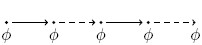
\includegraphics[scale=0.5]{graphics/Ltlalways.png}\\ 
$\diamondsuit \phi$ & $\phi$ has to hold \textbf{eventually} & 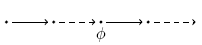
\includegraphics[scale=0.5]{graphics/Ltlevently.png}\\ 
$\bigcirc \phi$ & $\phi$ has to hold \textbf{next} & 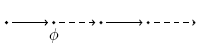
\includegraphics[scale=0.5]{graphics/Ltlnext.png}\\ 
$\psi\U\phi$ & $\psi$ has to hold at least \textbf{until} $\phi$ holds & 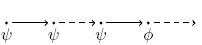
\includegraphics[scale=0.5]{graphics/Ltluntil.png}\\ 
\end{tabular}
\caption{\gls{LTL} quantifiers}
\label{tabl:ltl}
\end{table}


Using \gls{LTL} one can express temporal properties such as 
%
\textit{pointer p is never null}: $\square p (\neq \mbox{null})$ or 
%
\textit{program P finishes}, equivalently, 
%
	program counter reaches the return statement at line $l_k$: $\diamondsuit\pc = l_k$.



\begin{example}
Temporal logic studies problems like the one exposed below.

\label{Collatz:conjecture}

Let $f$ be the following function.

\[
f(n) = \left\{
	\begin{array}{cc}
		\rfrac{n}{2} & \text{ if } (n\text{ mod } 2) \equiv 0\\
		3n+1 & \text{ if } (n\text{ mod } 2) \equiv 1
	\end{array}
\right.
\]

We can form a sequence applying repeatedly $f$. If we take the sequence starting in $n=13$ we get:
%
\[ 
	13 \overset{\displaystyle\;\; 3n+1\;\;}{\longrightarrow}
	40 \overset{\displaystyle\;\;\rfrac{n}{2}\;\;}{\longrightarrow}
	20 \overset{\displaystyle\;\;\rfrac{n}{2}\;\;}{\longrightarrow}
	10 \overset{\displaystyle\;\;\rfrac{n}{2}\;\;}{\longrightarrow}
	5 \overset{\displaystyle\;\; 3n+1\;\;}{\longrightarrow}
	16 \overset{\displaystyle\;\;\rfrac{n}{2}\;\;}{\longrightarrow}
	8 \overset{\displaystyle\;\;\rfrac{n}{2}\;\;}{\longrightarrow}
	4 \overset{\displaystyle\;\;\rfrac{n}{2}\;\;}{\longrightarrow}
	2 \overset{\displaystyle\;\;\rfrac{n}{2}\;\;}{\longrightarrow}
	1
\]
%
One could ask if this sequence eventually stops regardless the integer chosen to begin. This question is called \concept{Collatz conjecture} and has not been solved yet. 
%
For the moment, an infinite sequence has not been found, but the temporal logic problem has not been proven either.
%

We could write in \gls{FOL} the formula for this conjecture as $[ \forall x \exists n (\underbrace{f \circ f \circ  ... \circ f}_{n})(x) = 1]$. However, the temporal formula for this problem is: $\diamondsuit \left(f(n) = 1\right)$
\end{example}


With \gls{LTL} one can express properties a program must hold to work properly. 
%
This properties may be \concept[Safety]{safety properties} or \concept[Liveness]{liveness properties}.

\label{def::safety}
\textbf{Safety properties} are ... \todo{Defn}

\label{def::liveness}
\textbf{Liveness properties} are ... \todo{Defn}


\gls{LTL} is a much wider field but just this introduction is needed to talk about formal verification.
